\begin{thm}{130}{\hosi 5}{東工大 (2019)}
 \begin{enumerate}
  \item $h>0$とする。座標平面上の点O$(0,0)$、点P$(h,s)$、点Q$(h,t)$に対して、$\triangle\mr{OPQ}$の面積を$S$とする。ただし$s<t$とする。$\triangle\mr{OPQ}$の辺OP, OQ, PQの長さをそれぞれ$p, q, r$とするとき、不等式
	\[ p^2+q^2+r^2\ge 4\sqrt{3}S \]
	が成り立つことを示せ。また、等号が成立するときの$s, t$の値を求めよ。 (Weitzenbockの不等式)
  \item 四面体ABCDの表面積を$T$、辺BC, CA, ABの長さをそれぞれ$a, b, c$とし、辺AD, BD, CDの長さをそれぞれ$l, m, n$とする。このとき、不等式
	\[a^2+b^2+c^2+l^2+m^2+n^2 \ge 2\sqrt{3}T \]
	が成り立つことを示せ。また、等号が成立するのは四面体ABCDがどのような四面体のときか。
 \end{enumerate}
\end{thm}

\syoumon{1}
\begin{wrapfigure}[9]{r}[0pt]{50pt}
 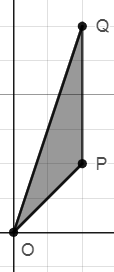
\includegraphics[width=\linewidth]{../problems/Q_130/A_130_1.png}
\end{wrapfigure}
$p=\sqrt{h^2+s^2}$, $q=\sqrt{h^2+t^2}$, $r=t-s$より、$p^2+q^2+r^2=2(h^2+t^2+s^2)-2st$。また右図より、$S=\dfrac{h}{2}(t-s)$。これらを用いて、
\begin{align*}
 &p^2+q^2+r^2-4\sqrt{3}S \\
 =&2(h^2+t^2+s^2)-2st-2\sqrt{3}h(t-s) \\
 =&2h^2-2\sqrt{3}(t-s)h+2(t^2+s^2-st)
\end{align*}
を得る。これを$h$の2次関数をみて$f(h)$とおくと、
\[ f(h)=2\left[h-\frac{\sqrt{3}}{2}(t-s)\right]^2+\frac{(t+s)^2}{2} \]
と整理できるから、$h=\dfrac{\sqrt{3}}{2}(t-s)$のときに最小値$\dfrac{(t+s)^2}{2}\ge 0$をとることがわかり、題意の不等式の成立が示された。さらに$f(h)$の最小値は、$t+s=0$のときに最小値0をとる。つまりこのとき与不等式の等号が成立し、このときの$s, t$の値は、$t+s=0$と$h=\dfrac{\sqrt{3}}{2}(t-s)$から、$s=-\dfrac{h}{\sqrt{3}}$, $t=\dfrac{h}{\sqrt{3}}$。

\syoumon{2}
(1)の結果により、
\begin{align*}
 a^2+b^2+c^2&\ge 4\sqrt{3}\triangle\mr{ABC} \\
 a^2+n^2+l^2&\ge 4\sqrt{3}\triangle\mr{ACD} \\
 c^2+m^2+l^2&\ge 4\sqrt{3}\triangle\mr{ABD} \\
 b^2+m^2+n^2&\ge 4\sqrt{3}\triangle\mr{BCD} \\
\end{align*}
となり、辺々足して、
\[ a^2+b^2+c^2+l^2+m^2+n^2 \ge 2\sqrt{3}T \qquad (\cdots \text{*}) \]
が示された。(*)で等号が成立することは、(1)を利用した4つの三角形全てにおいて等号が成立する場合と同値である。

\begin{wrapfigure}[12]{r}[0pt]{80pt}
 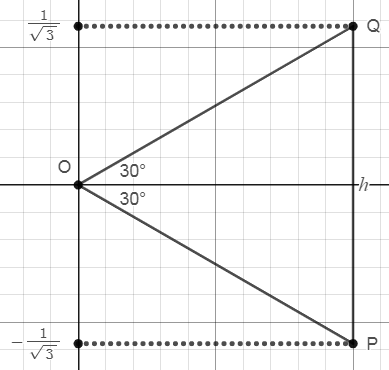
\includegraphics[width=\linewidth]{../problems/Q_130/A_130_2.png}
\end{wrapfigure}
翻って(1)の$\triangle\mr{OPQ}$において等号が成立する状況は、右図のようになっているから、$\angle\mr{POQ}=60^\circ$がわかる。また$\mr{OP}=\mr{OQ}$なので、$\triangle\mr{OPQ}$は正三角形である。\\
したがって、(*)で等号が成立することは、$\triangle\mr{ABC}$, $\triangle\mr{ACD}$, $\triangle\mr{ABD}$, $\triangle\mr{BCD}$が全て正三角形であることに同値である。1つの辺の長さを指定すれば、その辺の長さをもつ正三角形が4面を構成するとわかるので、等号の成立は正四面体のときである。